\documentclass{standalone}
\usepackage{tikz}
\usetikzlibrary{arrows.meta, positioning, fit, patterns, shapes.geometric}

\begin{document}
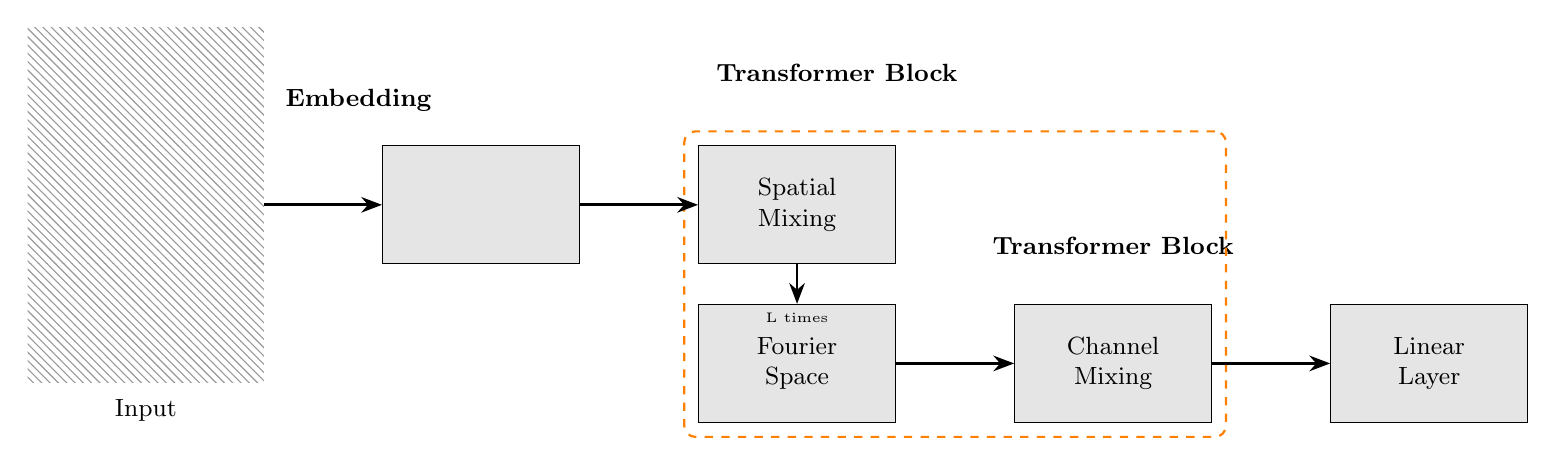
\begin{tikzpicture}[
  >=Stealth, % Arrow style
  node distance=1cm and 1.5cm, % Node distances
  box/.style={rectangle, draw, minimum width=2.5cm, minimum height=1.5cm, align=center, fill=gray!20}, % Box style
  transformer/.style={draw=orange, dashed, thick, rounded corners, inner sep=0pt, fit=#1}, % Transformer block style
  input-grid/.style={pattern=north west lines, pattern color=black!40, minimum width=3cm, minimum height=1.5cm, inner sep=0pt, outer sep=0pt}, % Input grid style
  font=\small % Font style
]

% Input
\node[input-grid] (grid-top) {};
\node[input-grid, below=0mm of grid-top] (grid-middle) {};
\node[input-grid, below=0mm of grid-middle] (grid-bottom) {};
\node[below=0.1cm of grid-bottom, anchor=north] (input-label) {Input};

% Embedding
\node[box, right=of grid-middle, label={[anchor=south east, xshift=-0.5cm, yshift=0.3cm]\textbf{Embedding}}] (embedding) {};

% Connection between input and embedding
\draw[->, line width=1pt] (grid-middle.east) --++ (0.8,0) |- (embedding.west);

% Transformer Block
\node[box, right=of embedding] (spatial-mixing) {Spatial\\Mixing};
\node[box, below=0.5cm of spatial-mixing] (fourier-space) {Fourier\\Space};
\node[box, right=of fourier-space] (channel-mixing) {Channel\\Mixing};
\node[above=0.5cm of channel-mixing, anchor=south] (transformer-label) {\textbf{Transformer Block}};
\node[below=0.5cm of spatial-mixing, anchor=north] (times-label) {\tiny L times};

% Transformer block fitting
\node[transformer=(spatial-mixing) (channel-mixing) (times-label), label={[anchor=south, xshift=-1.5cm, yshift=0.5cm]north:\textbf{Transformer Block}}, inner sep=5pt] {};

% Linear Layer
\node[box, right=of channel-mixing] (linear-layer) {Linear\\Layer};

% Arrows
\draw[->, line width=1pt] (embedding.east) -- (spatial-mixing.west);
\draw[->, line width=1pt] (spatial-mixing.south) -- (fourier-space.north);
\draw[->, line width=1pt] (fourier-space.east) -- (channel-mixing.west);
\draw[->, line width=1pt] (channel-mixing.east) -- (linear-layer.west);

\end{tikzpicture}
\end{document}